\begin{frame}
\frametitle{Aufgabe 3}
\framesubtitle{}
Im Oszilloskop wurden verschiedene Kennlinien von Bauteilen analysiert:
\begin{itemize}
    \item Kondensator
    \item Diode
    \item Spule
    \item LED
\end{itemize}
\end{frame}
\begin{frame}
\frametitle{Aufgabe 3}
\framesubtitle{Kennlinie Kondensator}
    \begin{figure}[H]
    \caption{Kondensator bei $69Hz$}
    \begin{center}
        \fbox{
            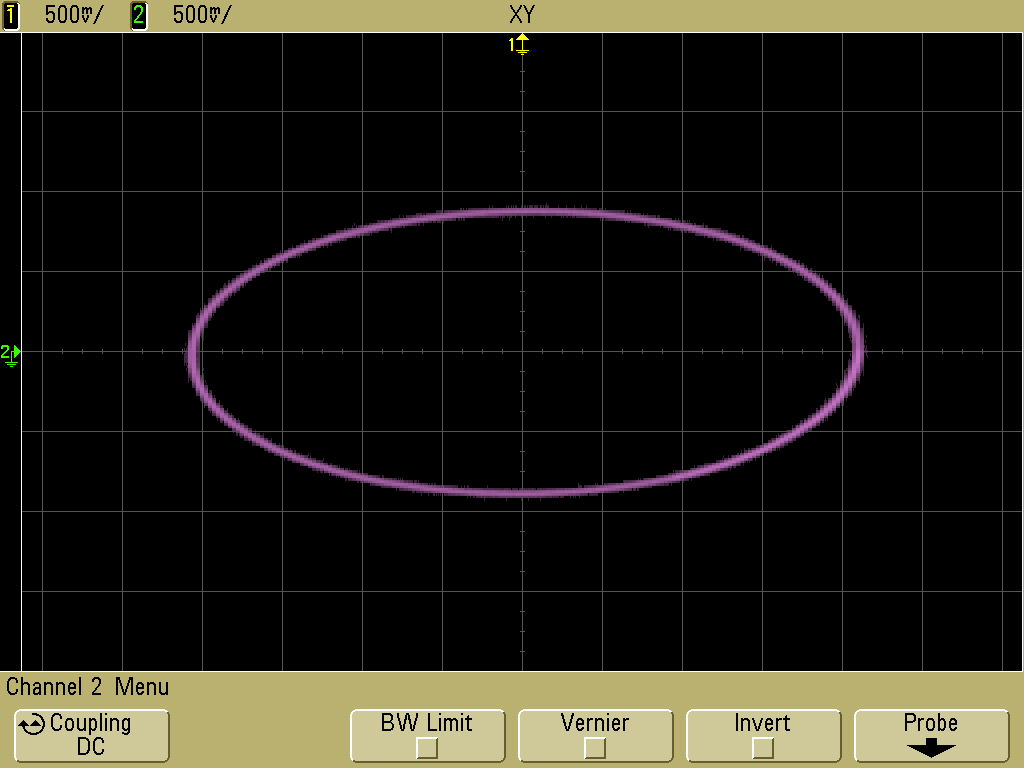
\includegraphics[scale=0.20]{./img/Kondensator_69_Hz.png}
        }
    \end{center}
    \end{figure}
\end{frame}
\begin{frame}
\frametitle{Aufgabe 3}
\framesubtitle{Kennlinie Kondensator}
\begin{itemize}
    \item hohe Frequenz $\rightarrow$ Gerade, Bauteil wird hoher Widerstand
    \item niedrige Frequenz: $\rightarrow$ Kreis/Elipsem Strom eilt Spannung durch Auf- und Entladen vorraus 
\end{itemize}
$\rightarrow$ Kondensator
\end{frame}
\begin{frame}
\frametitle{Aufgabe 3}
\framesubtitle{Kennlinie Diode}
    \begin{figure}[H]
    \caption{Diode bei $69Hz$}
    \begin{center}
        \fbox{
            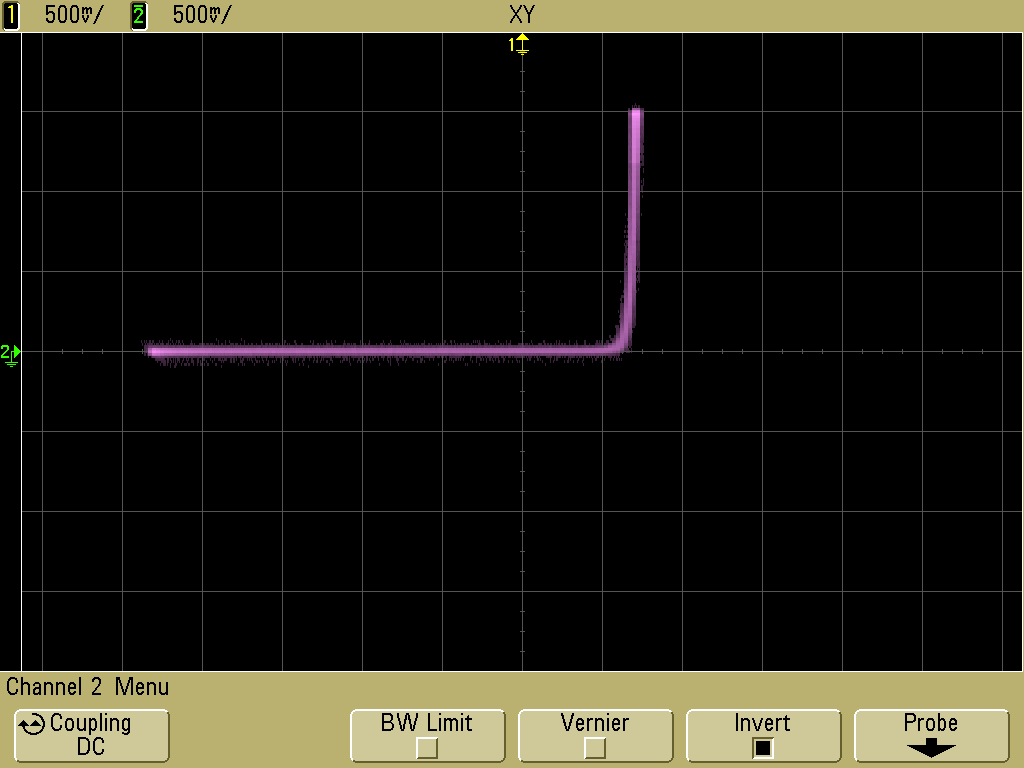
\includegraphics[scale=0.25]{./img/Diode_69_Hz.png}
        }
    \end{center}
    \end{figure}
\end{frame}
\begin{frame}
\frametitle{Aufgabe 3}
\framesubtitle{Kennlinie Diode}
    \begin{itemize}
        \item Kennlinie ist Null bis Sperrspannung überschritten ist
        $\rightarrow$ Diode oder LED
    \end{itemize}
\end{frame}
\begin{frame}
\frametitle{Aufgabe 3}
\framesubtitle{Kennlinie Diode}
    \begin{center}
        Einfluss des eingebauten Kondensators bei hohen Frequenzen:
    \end{center}
    \begin{figure}[H]
    \begin{center}
        \fbox{
            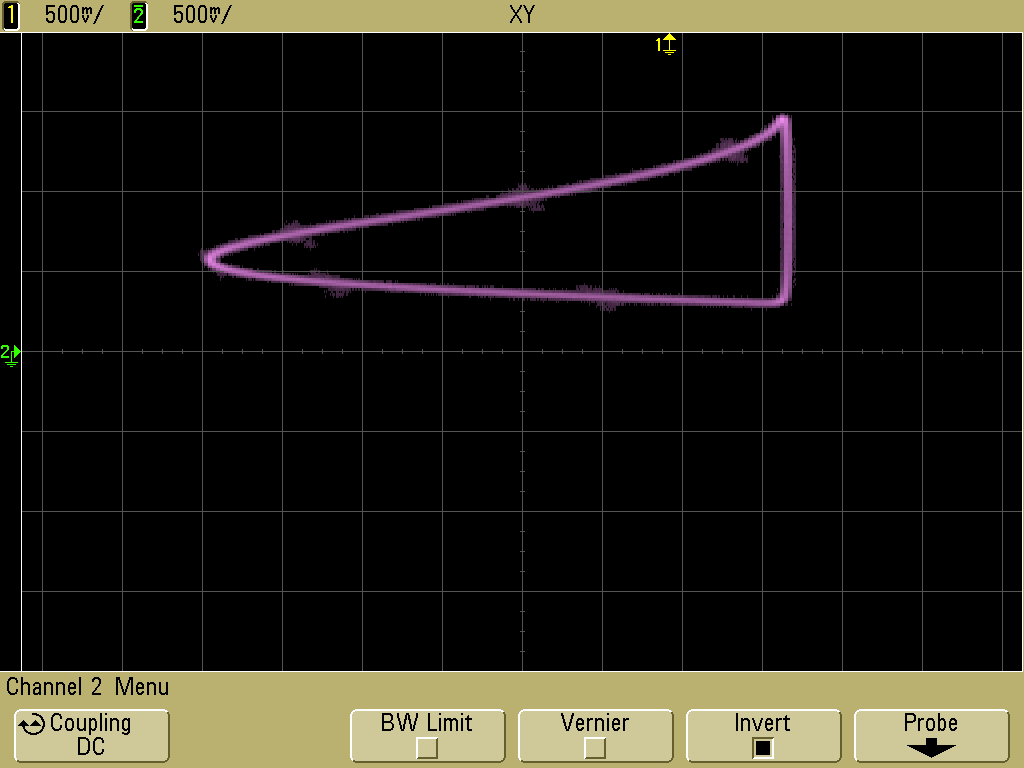
\includegraphics[scale=0.20]{./img/Kondensatorlinie_bei_Diode.png}
        }
    \end{center}
    \end{figure}
    
\end{frame}
\begin{frame}
\frametitle{Aufgabe 3}
\framesubtitle{Kennlinie Diode}
    \begin{center}
    Diodenkennlinie bei höheren Frequenzen.
    \end{center}
    \begin{figure}[H]
        \begin{center}
            \fbox{
                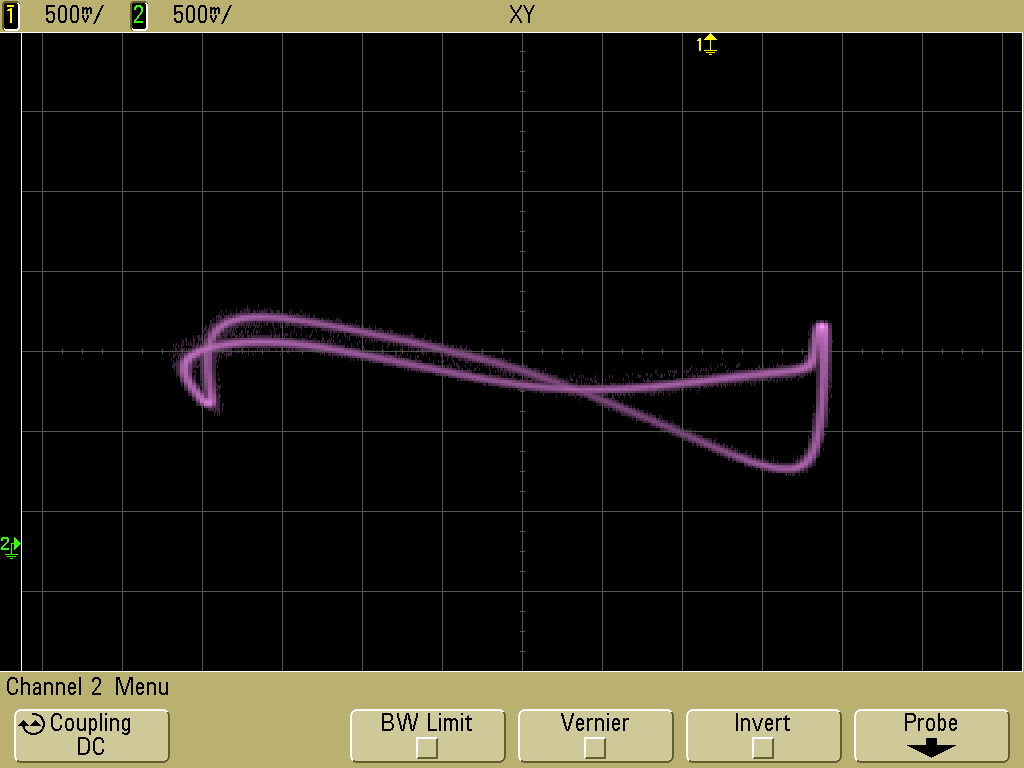
\includegraphics[scale=0.20]{./img/Diode_1_MHz.png}
            }
        \end{center}
    \end{figure}
\end{frame}
\begin{frame}
\frametitle{Aufgabe 3}
\framesubtitle{Kennlinie Diode}
    \begin{figure}[H]
        \begin{center}
            \fbox{
                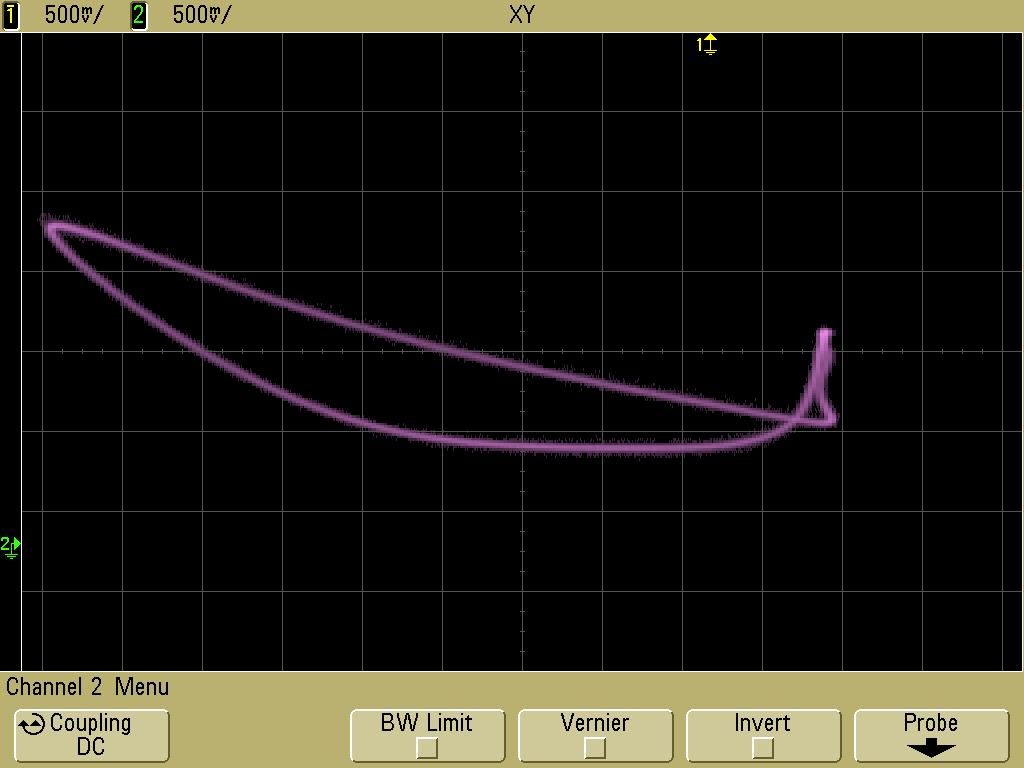
\includegraphics[scale=0.20]{./img/Diode_2_MHz.png}
            }
        \end{center}
    \end{figure}
\end{frame}
\begin{frame}
\frametitle{Aufgabe 3}
\framesubtitle{Kennlinie Diode}
    \begin{figure}[H]
        \begin{center}
            \fbox{
                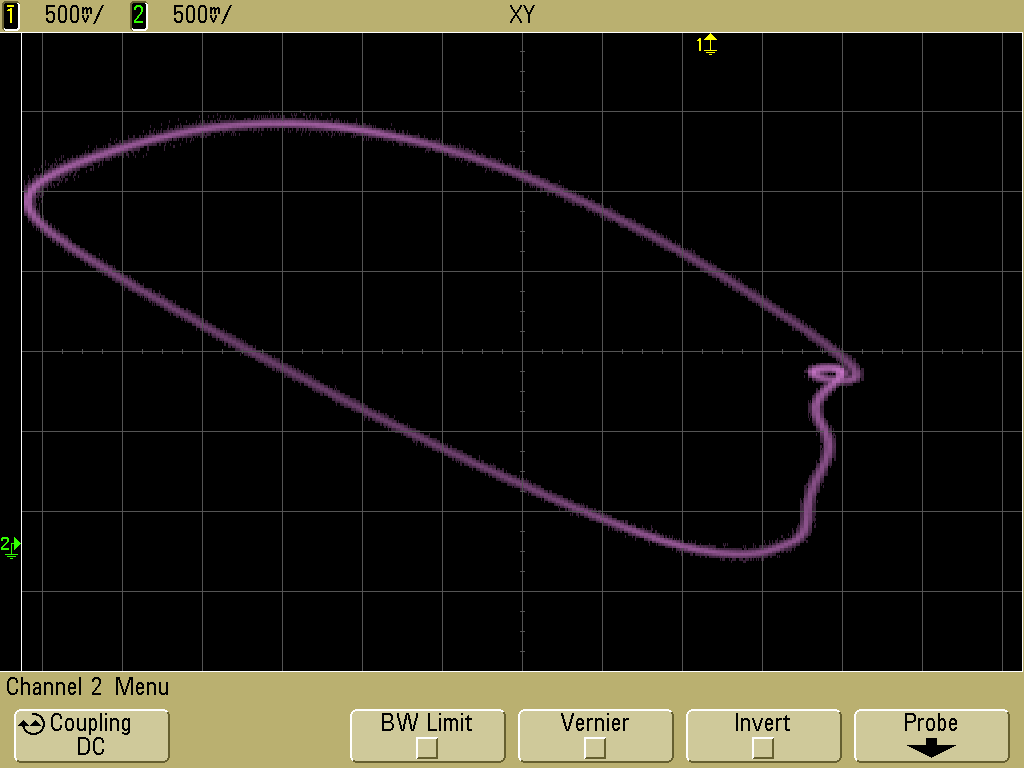
\includegraphics[scale=0.20]{./img/Diode_3_MHz.png}
            }
        \end{center}
    \end{figure}
    $\rightarrow$ Kennlinie wird durch Bauelemente in Quelle und Messgerät
    stark verfälscht.
\end{frame}

\begin{frame}
\frametitle{Aufgabe 3}
\framesubtitle{Kennlinie Spule}
    \begin{figure}[H]
    \begin{center}
        \fbox{
            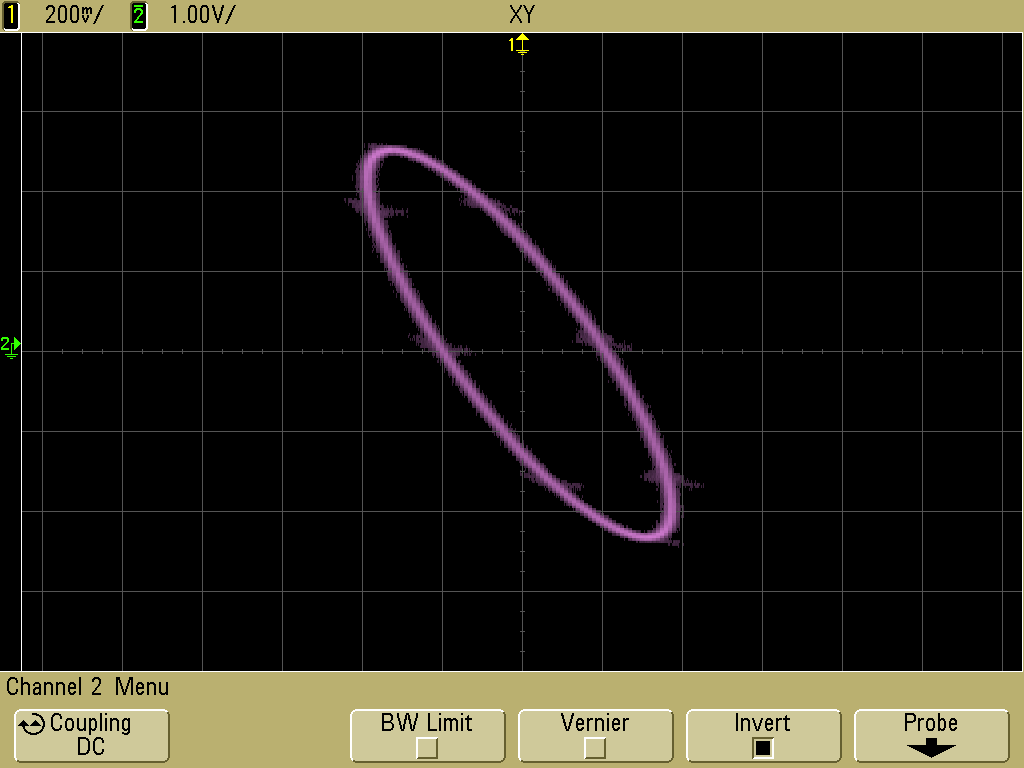
\includegraphics[scale=0.25]{./img/Spule_9_kHz.png}
        }
    \end{center}
    \end{figure}
\end{frame}
\begin{frame}
\frametitle{Aufgabe 3}
\framesubtitle{Kennlinie Spule}
\begin{itemize}
    \item hohe Frequenz $\rightarrow$ Gerade, Bauteil wird hoher Widerstand
    \item niedrige Frequenz: $\rightarrow$ Phasenverschiebung durch
    Induktivität
\end{itemize}
$\rightarrow$ Spule
\end{frame}
\begin{frame}
\frametitle{Aufgabe 3}
\framesubtitle{Kennlinie LED}
    \begin{figure}[H]
    \begin{center}
        \fbox{
            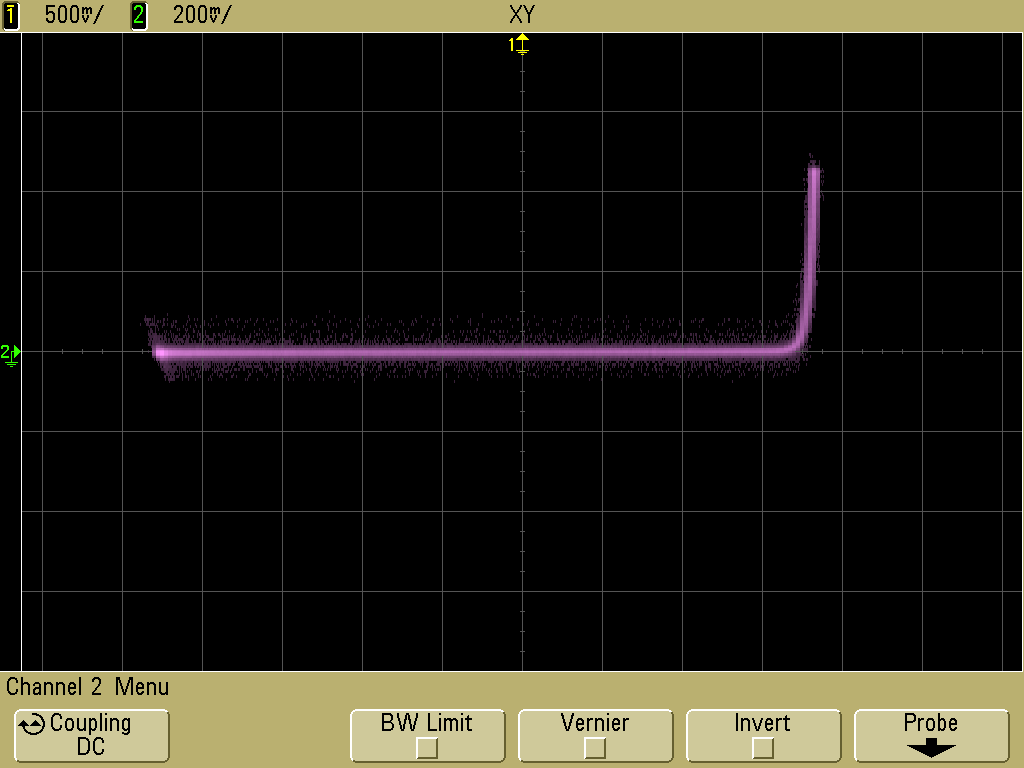
\includegraphics[scale=0.25]{./img/LED_30_Hz.png}
        }
    \end{center}
    \end{figure}

\end{frame}
\begin{frame}
\frametitle{Aufgabe 3}
\framesubtitle{Kennliie LED}
\begin{itemize}
    \item Kennlinie wie Diode
    \item Kein erkennbarer Unterschied
    $\rightarrow$ durch einen größeren Spannungsbereich hätte eventuell die
    Diode von der LED unterschieden werden können (früheres Abfallen im
    negativen)
\end{itemize}
\end{frame}
